\documentclass[12pt,a4paper,notitlepage]{article}

\usepackage{latexsym}
\usepackage[MeX]{polski}
\usepackage[utf8]{inputenc}
\usepackage{graphicx}
\usepackage{listings}
\usepackage{amsmath}

\usepackage[top=2cm, bottom=2cm, left=3cm, right=3cm]{geometry}

\makeatletter

\newcommand{\linia}{\rule{\linewidth}{0.4mm}}

\renewcommand{\maketitle}{\begin{titlepage}

    \vspace*{1cm}

    \begin{center}\small

   	 Politechnika Warszawska\\
    	Wydział Mechatroniki\\
 	Instytut Automatyki i Robotyki
    \end{center}
    \vspace{3cm}


    \begin{center}

	\small
	Programowanie w języku Java \\
	Projekt ćwiczeniowy \\
	
      \LARGE \textsc{Odtwarzacz i edytor muzyki}

         \end{center}


    \vspace{5.5cm}

    \begin{flushright}

    \begin{minipage}{5cm}

    \textit{\small Autorzy:}\\

    \normalsize \textsc{Konrad Traczyk} \par
    \normalsize \textsc{Jakub Szlendak} \par

    \end{minipage}

    \vspace{5cm}

     {\small Prowadzący:}\\
 
         {prof. dr hab. Barbara Siemiątkowska}\\	
         {mgr. inż Irina Gorbenko}

     \end{flushright}

    \vspace*{\stretch{6}}

    \begin{center}

    \@date

    \end{center}

  \end{titlepage}%

}

\makeatother

\begin{document}

\maketitle

\section{Wstęp}
\label{sec:wstep}

Przedmiotem projektu było zaprojektowanie aplikacji odtwarzającej pliki muzyczne z funkcją edycji w języku programowania Java. Ustalono następujące wymagania co do funkcjonalności:
\begin{itemize}
 \item odtwarzanie plików w formacie MP3 i WAVE
 \item edycja plików w obydwu formatach
 \item realizacja podstawowych operacji edycyjnych - skracanie ścieżki muzycznej, wycinanie fragmentu ścieżki, modyfikacja poszczególnych próbek w ścieżce
 \item obsługa listy odtwarzania
 \item obsługa kilku trybów odtwarzania (pojedyncza piosenka, powtarzanie piosenki itp.)
\end{itemize}

\section{Implementacja aplikacji}
\label{sec:implementacja}
Podstawowym elementem odtwarzacza muzyki jest silnik dekodujący pliki MP3. Biblioteki standardowe języka Java nie dostarczają takiej funkcjonalności.
Ponieważ zaimplementowanie dekodowania ramek pliku MP3 jest zadaniem złożonym i wykraczającym poza zakres merytoryczny tego projektu, wykorzystano do tego bibliotekę JLayer dostarczaną na licencji 
GPL przez firmę JavaZoom. Z wspomnianej biblioteki wykorzystano dekoder ramek MP3 oraz konwerter plików MP3 na format WAVE. Klasa odtwarzacza dostarczana przez wymienioną bibliotekę została zmodyfikowana do potrzeb projektu. 

Program był rozwijany jednocześnie na dwóch systemach operacyjnych: Windows 7 oraz Linux Ubuntu 14.04. Jego implementacja nie jest zależna od systemu operacyjnego, jest to zatem aplikacja wieloplatformowa. 

\section{Algorytm odtwarzania}
\label{sec:odtwarzanie}
Za odtwarzanie muzyki odpowiadają klasy \emph{AdvancedPlayer} i \emph{Player}.   
Jak wspomniano wcześniej, klasa odtwarzacza (AdvancedPlayer), należąca do biblioteki JLayer, została zmodyfikowana na potrzeby projektu. Modyfikacja polegała na zmianach w funkcji odtwarzającej tak, 
aby możliwe było odtwarzanie od dowolnej ramki. Działanie funkcji odtwarzającej polega na dekodowaniu i odtwarzaniu kolejnych ramek pliku w pętli, aż odtworzona zostanie ostatnia ramka
bądź proces zostanie przerwany ręcznie. 

Klasa \emph{Player} opakowuje odwarzanie pliku w dodatkowe funkcjonalności - odtwarzanie od zadanego momentu, pauza, stop itp. Dodatkowo, obsługuje listę odtwarzania.
Lista odtwarzania została zamodelowana jako kolekcja typu \emph{LinkedList}. Pozwala to na wydajne operacje modyfikacji kolejności bądź wstawiania elementów.

Na liście agregowane są 
obiekty klasy \emph{PlaylistItem}, zawierające obiekt klasy \emph{File} przechowujący referencję do pliku muzycznego oraz napisy zawierające metadane piosenki, odczytane z pliku. Metadane są 
odczytywane podczas tworzenia obiektu klasy \emph{PlaylistItem}. Jeżeli nie uda się odczytać metadanych, przyjmuje się że tytułem piosenki jest nazwa pliku, a pozostałe pola są puste. 
Podejmowana jest także próba odczytania pliku graficznego w folderze z piosenką - jeżeli znajduje się w nim jakiś plik graficzny, jest on traktowany jako okładka albumu. 

\section{Algorytm edycji}
\label{sec:edycja}
Zaimplementowano następujące możliwości edycji pliku muzycznego:
\begin{itemize}
 \item konwersja pliku MP3 do formatu WAVE
 \item wyciszanie fragmentu pliku o zadanej długości i początku
 \item wycinane zadanego fragmentu pliku (``przycinanie'' piosenki)
 \item zmiana głośności piosenki
\end{itemize}
Ponieważ edycję przeprowadza się na poszczególnych próbkach w pliku muzycznym, konieczne jest operowanie na plikach nieskompresowanych. Dlatego operacje edycyjne w programie przeprowadzane są na plikach WAVE. Możliwe jest załadowanie do edytora pliku w formacie MP3, ale zostanie on przekonwertowany do tymczasowego pliku WAVE umieszczonego w folderze programu. Po zakończeniu edycji plik tymczasowy jest usuwany. Nalezy także nadmienić, że plik źródłowy nie jest modyfikowany podczas edycji.

Operacje edycyjne rozpoczynają się od pobrania nagłówka pliku WAVE. Zawarte są w nim informacje takie jak:
\begin{itemize}
 \item format pliku
 \item liczba kanałów
 \item bitrate i sample rate (liczba bitów i próbek na sekundę)
\end{itemize}
W nagłówku zawarta jest także informacja o pozycji bajtowej pierwszej próbki. Ta pozycja jest pobierana i traktowana jako początek danych o dźwięku. Mając tę informację, można poruszać się po pliku jak po tablicy typu \textbf{byte}. Należy przy tym pamiętać, że pojedyncza próbka zapisana jest na dwóch bajtach. Modyfikacja zawartości komórek tej tablicy wpływa na dźwięk. 

W konsekwencji, wyciszanie fragmentu piosenki polega na wyzerowaniu pewnej ilości próbek, zaś zmiana głośności na przemnożeniu ich przez współczynnik. 

Z kolei wycinanie fragmentu piosenki polega na wycięciu części bajtów i wstawieniu ich do strumienia wyjściowego, odpowiednio modyfikując nagłówek.

\section{Interfejs użytkownika}
\label{sec:Interfejs}
Interfejs użytkownika został zaimplentowany przy użyciu biblioteki Swing.

\begin{figure}[hb]
 \centering
 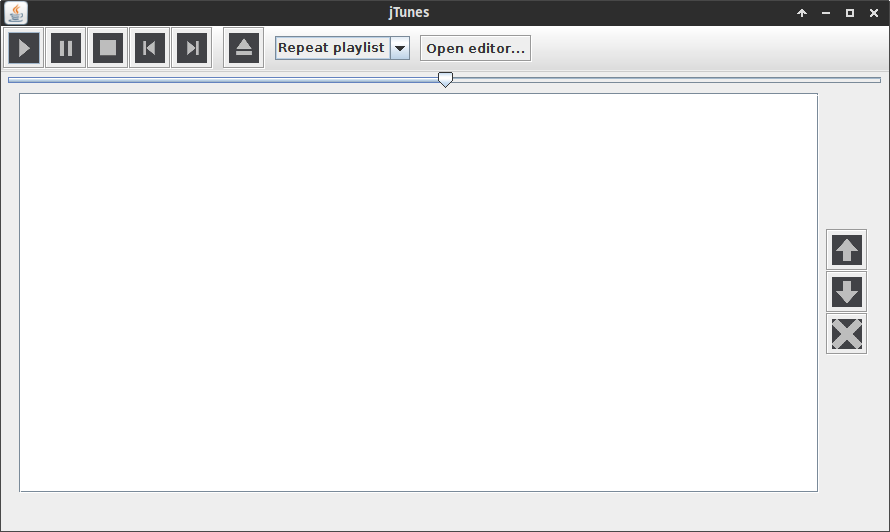
\includegraphics[width=0.9\textwidth]{img/player_blank.png}
 \caption{Okno główne programu}
 \label{fig:player_blank}
\end{figure}

Rysunek \ref{fig:player_blank} przedstawia okno programu tuż po jego załadowaniu. Program jest w trybie odtwarzania. W górnej części okna widoczny jest pasek narzędzi odtwarzania. Funkcje kolejnych
przycisków:
\begin{itemize}
 \item rozpoczęcie odtwarzania
 \item pauza
 \item zatrzymanie odtwarzania
 \item następna piosenka z listy
 \item poprzednia piosenka z listy
 \item przycisk otwierania plików
 \item lista rozwijana trybów odtwarzania
 \item przycisk przełączenia na tryb edycji
\end{itemize}
Pod paskiem narzędzi umiejscowiono wskaźnik postępu odtwarzania, zaś poniżej znajduje się panel listy odtwarzania (por. rys. \ref{fig:player_playing}).

Poszczególne pozycje na liście zawierają okładkę albumu (jeśli została znaleziona, w przeciwnym razie wyświetlany jest obrazek domyślny), metadane piosenki (kolejno: wykonawcę, 
album i tytuł, bądź nazwę pliku jeśli metadane nie są dostępne) oraz długość piosenki w minutach i sekundach. Za wyświetlanie tych informacji odpowiada klasa \emph{PlaylistItemRenderer}.

Po prawej stronie panelu listy odtwarzania umieszczono przyciski manipulowania listą. Pozwalają one na przesuwanie zaznaczonego elementu playlisty do góry, w dół bądź usuwanie go.

Aby rozpocząć odtwarzanie należy klikąć przycisk ,,Otwórz'', a następnie wybrać co najmniej jeden plik muzyczny do otwarcia (możliwe jest wybranie wielu plików, patrz rys. \ref{fig:open}).
Wybrane pliki zostają dodane do listy odtwarzania. Następnie należy wybrać jedną z 4 opcji porządku odtwarzania za pomocą listy rozwijanej:
\begin{description}
 \item[Repeat playlist] odtwarzanie w porządku listy - piosenki z listy są odtwarzana kolejno, gdy osiągnięty zostanie koniec listy, odtwarzanie jest przenoszone na początek
 \item[Shuffle playlist] odtwarzanie losowe z listy - piosenki z listy są odtwarzane w losowej kolejności
 \item[Play single] odwarzanie zaznaczonej piosenki, po osiągnięciu końca piosenki otwarzanie zostaje zakończone
 \item[Repeat single] zaznaczona piosenka jest odwarzana w pętli
\end{description}
Po wybraniu trybu odtwarzania można rozpocząć otwarzanie przyciskiem ,,Odtwarzaj'' lub przez dwukrotne kliknięcie piosenki na liście.

\begin{figure}[hb]
 \centering
 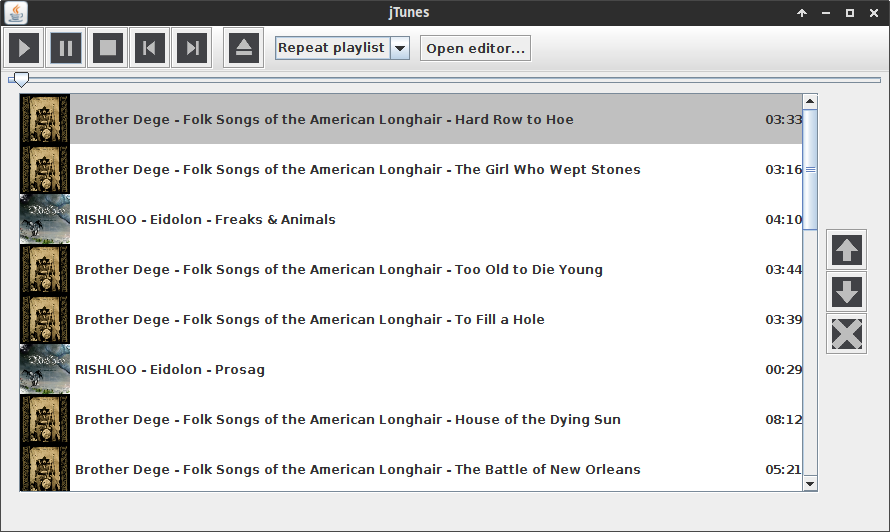
\includegraphics[width=0.9\textwidth]{img/player_playing.png}
 \caption{Okno główne programu podczas odtwarzania}
 \label{fig:player_playing}
\end{figure}

\begin{figure}[hb]
 \centering
 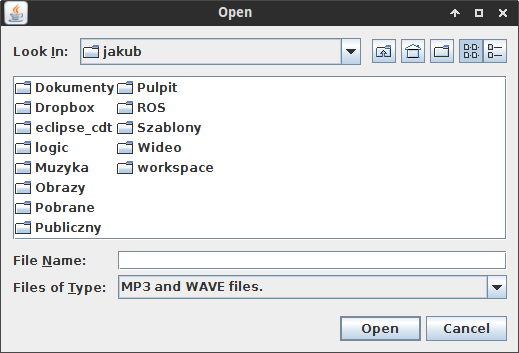
\includegraphics[width=0.6\textwidth]{img/open.png}
 \caption{Okno otwierania pliku}
 \label{fig:open}
\end{figure}

Po wybraniu przycisku edycji otwarty zostaje widok edycji (por. rys. \ref{fig:editor}). Przyciski odtwarzania są nadal dostępne i odtwarzanie może być kontynuowane. W panelu edycji widoczne
są cztery sekcje:
\begin{itemize}
 \item przyciski otwierania i zapisu pliku
 \item kontrolki do przycinania pliku
 \item kontrolki do wyciszania fragmentu pliku
 \item kontrolki do zmiany głośności pliku
\end{itemize}

Przyciski edycyjne są nieaktywne do momentu załadowania pliku za pomocą przycisku ,,Open file''. Po zakończeniu edycji plik można zapisać za pomocą przycisku ,,Save file''. 
W celu wykonania przycięcia bądź wyciszenia piosenki, należy wpisać w odpowiednie pola edycyjne moment początku i końca modyfikacji (w sekundach). Modyfikacja głośności sprowadza się do 
wybrania nowej głośności (w procentach) i kliknięcia przycisku ,,Change volume''. Możliwe jest wykonanie kliku operacji edycyjnych na jedno załadowanie pliku.

\begin{figure}[hb]
 \centering
 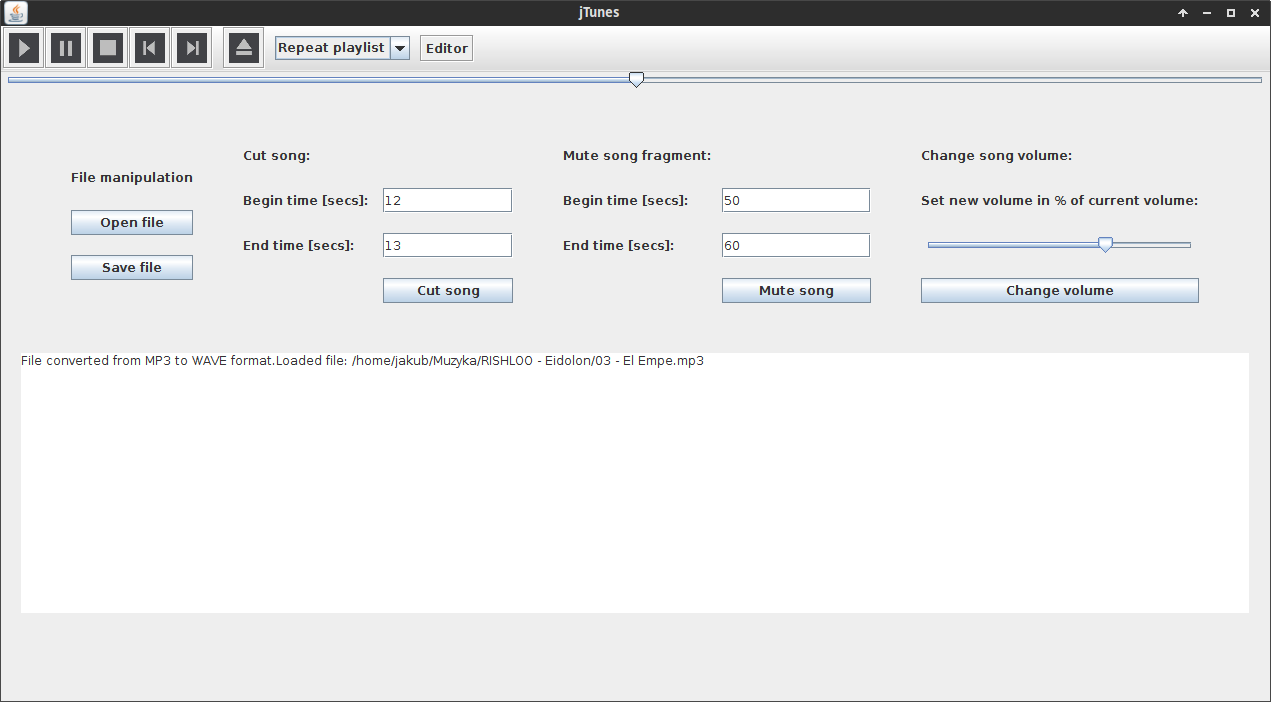
\includegraphics[width=0.9\textwidth]{img/editor.png}
 \caption{Ekran edycji}
 \label{fig:editor}
\end{figure}

\begin{figure}[hb]
 \centering
 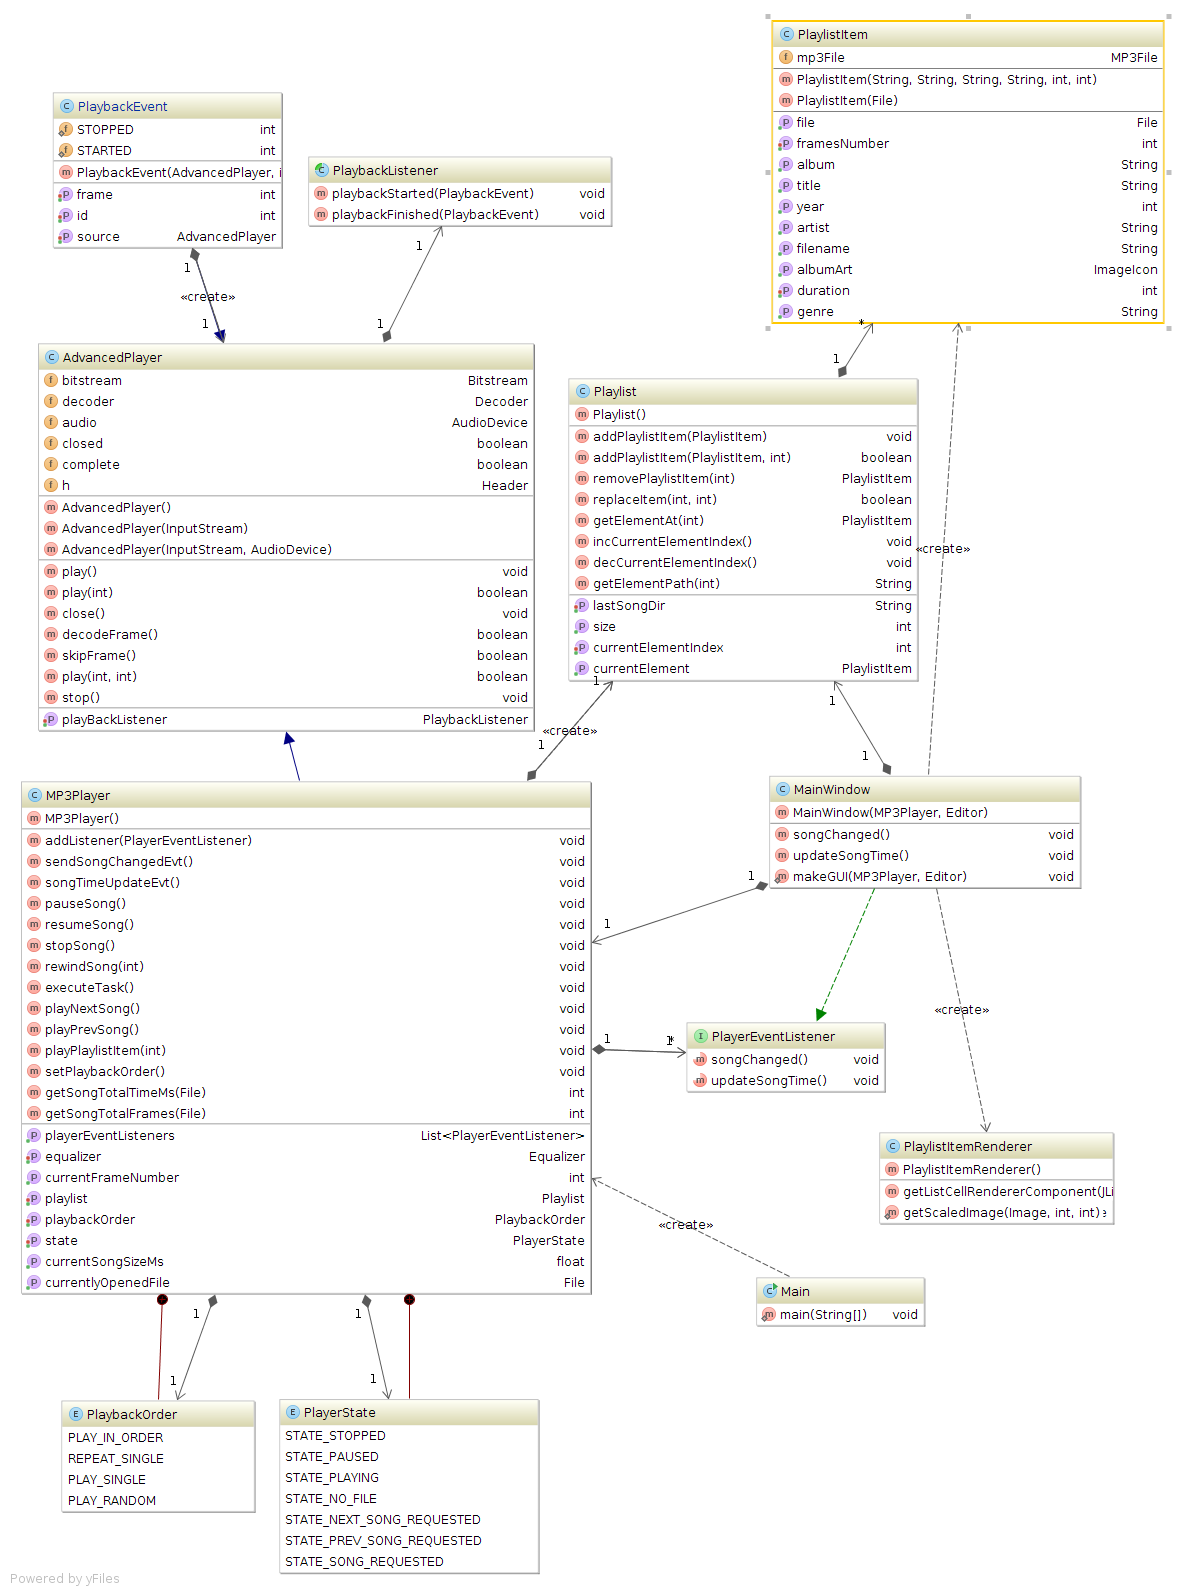
\includegraphics[width=1.1\textwidth]{img/diagram.png}
\end{figure}



\end{document}


























 
